\documentclass[12pt,a4paper]{article}
\usepackage{amsmath,amssymb,mathrsfs,tikz,times,pifont}
\usepackage{enumitem}
\usetikzlibrary{positioning}%Pour l'arbre de proba
\newcommand\circitem[1]{%
\tikz[baseline=(char.base)]{
\node[circle,draw=gray, fill=red!55,
minimum size=1.2em,inner sep=0] (char) {#1};}}
\newcommand\boxitem[1]{%
\tikz[baseline=(char.base)]{
\node[fill=cyan,
minimum size=1.2em,inner sep=0] (char) {#1};}}
\setlist[enumerate,1]{label=\protect\circitem{\arabic*}}
\setlist[enumerate,2]{label=\protect\boxitem{\alph*}}
%%%::::::by chnini ameur :::::::%%%
\everymath{\displaystyle}
\usepackage[left=1cm,right=1cm,top=1cm,bottom=1.7cm]{geometry}
\usepackage[colorlinks=true, linkcolor=blue, urlcolor=blue, citecolor=blue]{hyperref}
\usepackage{array,multirow}
\usepackage[most]{tcolorbox}
\usepackage{varwidth}
\usepackage{float} %pour utiliser l'option [H] qui force l'image à apparaître exactement à l'endroit où elle est placée dans le code.
\tcbuselibrary{skins,hooks}
\usetikzlibrary{patterns}
%%%::::::by chnini ameur :::::::%%%
\newtcolorbox{exa}[2][]{enhanced,breakable,before skip=2mm,after skip=5mm,
colback=yellow!20!white,colframe=black!20!blue,boxrule=0.5mm,
attach boxed title to top left ={xshift=0.6cm,yshift*=1mm-\tcboxedtitleheight},
fonttitle=\bfseries,
title={#2},#1,
% varwidth boxed title*=-3cm,
boxed title style={frame code={
\path[fill=tcbcolback!30!black]
([yshift=-1mm,xshift=-1mm]frame.north west)
arc[start angle=0,end angle=180,radius=1mm]
([yshift=-1mm,xshift=1mm]frame.north east)
arc[start angle=180,end angle=0,radius=1mm];
\path[left color=tcbcolback!60!black,right color = tcbcolback!60!black,
middle color = tcbcolback!80!black]
([xshift=-2mm]frame.north west) -- ([xshift=2mm]frame.north east)
[rounded corners=1mm]-- ([xshift=1mm,yshift=-1mm]frame.north east)
-- (frame.south east) -- (frame.south west)
-- ([xshift=-1mm,yshift=-1mm]frame.north west)
[sharp corners]-- cycle;
},interior engine=empty,
},interior style={top color=yellow!5}}
%%%%%%%%%%%%%%%%%%%%%%%

\usepackage{fancyhdr}
\usepackage{eso-pic}         % Pour ajouter des éléments en arrière-plan
% Commande pour ajouter du texte en arrière-plan
\usepackage{tkz-tab}
\AddToShipoutPicture{
    \AtTextCenter{%
        \makebox[0pt]{\rotatebox{80}{\textcolor[gray]{0.7}{\fontsize{5cm}{5cm}\selectfont PGB}}}
    }
}
\usepackage{lastpage}
\fancyhf{}
\pagestyle{fancy}
\renewcommand{\footrulewidth}{1pt}
\renewcommand{\headrulewidth}{0pt}
\renewcommand{\footruleskip}{10pt}
\fancyfoot[R]{
\color{blue}\ding{45}\ \textbf{2024}
}
\fancyfoot[L]{
\color{blue}\ding{45}\ \textbf{Prof:M. BA}
}
\cfoot{\bf
\thepage /
\pageref{LastPage}}

% Définition de l'encadré adaptatif avec fond jaune
\newtcolorbox{resultbox}{
    colback=red!30, % Fond rouge clair
    colframe=black, % Bordure noire fine
    sharp corners, % Coins nets
    boxrule=0.5pt, % Contour léger
    boxsep=2pt, % Espacement interne
    left=5pt, right=5pt, top=2pt, bottom=2pt, % Marges internes
}

\begin{document}
\renewcommand{\arraystretch}{1.5}
\renewcommand{\arrayrulewidth}{1.2pt}
\begin{tikzpicture}[overlay,remember picture]
    \node[draw=blue,line width=1.2pt,fill=purple,text=blue,inner sep=3mm,rounded corners,pattern=dots]at ([yshift=-2.5cm]current page.north) {\begingroup\setlength{\fboxsep}{0pt}\colorbox{white}{\begin{tabular}{|*1{>{\centering \arraybackslash}p{0.28\textwidth}} |*2{>{\centering \arraybackslash}p{0.2\textwidth}|} *1{>{\centering \arraybackslash}p{0.19\textwidth}|} }
                \hline
                \multicolumn{3}{|c|}{$\diamond$$\diamond$$\diamond$\ \textbf{Lycée de Dindéfélo}\ $\diamond$$\diamond$$\diamond$ } & \textbf{A.S. : 2024/2025}                                                              \\ \hline
                \textbf{Matière: Mathématiques}                                                                                    & \textbf{Niveau : T}\textbf{S2} & \textbf{Date: 09/12/2024} & \textbf{Durée : 4 heures} \\ \hline
                \multicolumn{4}{|c|}{\parbox[c]{10cm}{\begin{center}
                                                                  \textbf{{\Large\sffamily Correction du devoir n$ ^{\circ} $ 1 Du 1$ ^\text{\bf er} $ Semestre}}
                                                              \end{center}}}                                                                                                                        \\ \hline
            \end{tabular}}\endgroup};
\end{tikzpicture}
\vspace{3cm}

\section*{\underline{Exercice 1 :} 5.5 points (BAC 2008)}

\section*{\underline{Exercice 1 :} 5.5 points (BAC 2008)}
\textbf{A)} 
\begin{enumerate}
    \item Si la première boule tirée est verte, on la met dans $U_2$.\\
Dans ce cas, $U_2$ comporte maintenant 5 boules vertes $V$ et 5 boules jaunes $J$.\\
On a par conséquent : 
\[
p(V_2 \mid V_1) = \frac{5}{10} \Rightarrow p(V_2 \mid V_1) = \frac{1}{2}
\]

\item  De même,
\[
p(V_2 \mid R_1) = \frac{1}{11}
\]

\item  Dressons un arbre pondéré de la situation.

\begin{tikzpicture}[xscale=3.5, yscale=2]
% Nœuds de départ
\node (D) at (0,0) {Départ};

% Niveau 1
\node (V1) at (1,1) {V};
\node (R1) at (1,-1) {R};

% Niveau 2
\node (VV) at (2,1.5) {V};
\node (VJ) at (2,0.5) {J};
\node (RJ) at (2,-0.2) {J};
\node (RR) at (2,-1.2) {R};
\node (RV) at (2,-3) {V};

% Branches départ
\draw (D) -- (V1) node[midway, left] {\(\frac{3}{5}\)};
\draw (D) -- (R1) node[midway, left] {\(\frac{2}{5}\)};

% Branches de V
\draw (V1) -- (VV) node[midway, above left] {\(\frac{1}{2}\)};
\draw (V1) -- (VJ) node[midway, below left] {\(\frac{1}{2}\)};

% Branches de R
\draw (R1) -- (RJ) node[midway, above left] {\(\frac{5}{11}\)};
\draw (R1) -- (RR) node[midway, left] {\(\frac{5}{11}\)};
\draw (R1) -- (RV) node[midway, below left] {\(\frac{1}{11}\)};

\end{tikzpicture}

D'après la formule des probabilités totales, 
\[
p(V_2) = p(V_2 \mid V_1) p(V_1) + p(V_2 \mid R_1) p(R_1)
\]
Soit :
\[
p(V_2) = \frac{1}{2} \times \frac{3}{5} + \frac{1}{11} \times \frac{2}{5} \Rightarrow p(V_2) = \frac{37}{110}
\]

\item  De manière analogue,
\[
p(J_2) = p(J_2 \mid V_1) p(V_1) + p(J_2 \mid R_1) p(R_1)
\]
\[
= \frac{1}{2} \times \frac{3}{5} + \frac{1}{11} \times \frac{2}{5}
\]
\[
= \frac{53}{110}
\]
On trouve :
\[
p(J_2) = \frac{53}{110}
\]

\item  De manière analogue à la question 3, on a :
\[
p(R_2) = p(R_2 \mid V_1) p(V_1) + p(R_2 \mid R_1) p(R_1)
\]
\[
= 0 + \frac{5}{11} \times \frac{2}{5}
\]
\[
= \frac{2}{11}
\]
On trouve :
\[
p(R_2) = \frac{2}{11}
\]
\end{enumerate}

\textbf{B)}
\begin{enumerate}
    \item  La loi de probabilité de $X$ est donnée par le tableau suivant :

\[
\begin{array}{|c|c|c|c|}
\hline
X & 1000 & 500 & -500 \\
\hline
p(X) & \frac{37}{110} & \frac{53}{110} & \frac{2}{11} \\
\hline
\end{array}
\]

\item 
\[
E(X) = \sum x_i p_i
\]
\[
E(X) = \left(1000 \times \frac{37}{110}\right) + \left(500 \times \frac{53}{110}\right) - \left(500 \times \frac{2}{11}\right)
\]
\[
E(X) = \frac{5350}{11}
\]

Donc, 
\[
E(X) = \frac{5350}{11}
\]
\end{enumerate}

\textbf{C)}
\begin{enumerate}
    \item On a affaire à un schéma de Bernoulli, la probabilité du succès étant $p(E) = \frac{37}{110}$ et le nombre d'épreuves étant 15.\\
La probabilité d'avoir exactement 8 succès est :
\[
P_8 = C_8^{15} \left( \frac{37}{110} \right)^8 \left( \frac{73}{110} \right)^7
\]

\textbf{2)} C'est l'événement : $\underbrace{\text{SSSSSSSS}}_{\text{8 fois}} \quad 
\underbrace{\text{EEEEEEE}}_{\text{7 fois}}$ (8 succès consécutifs suivis de 7 échecs consécutifs).\\
Sa probabilité est :
\[
p(S)^8 \times p(E)^7 = \left( \frac{37}{110} \right)^8 \times \left( \frac{73}{110} \right)^7 \approx 9.310^{-6}
\]

\textbf{3)} L'événement contraire est : 
\[
P_0 = C_0^{15} \left( \frac{37}{110} \right)^0 \left( \frac{73}{110} \right)^{15}
\]
La probabilité cherchée est donc :
\[
\begin{aligned}
    p &= 1 - P_0\\
    &= 1 - \left( \frac{73}{110} \right)^{15}\\
    &\approx 0.997
\end{aligned}
\]
\end{enumerate}
\section*{\underline{Problème :} 9,5 points (BAC 2007)}
\subsection*{\underline{\textbf{Partie A}}:\textbf{ 3 pts}}
Soit $g$ la fonction définie sur $]0 ; +\infty[$ par :
\[
g(x) = 1 + x + \ln x
\]

\begin{enumerate}
    \item Dressons le tableau de variation de $g$.

Soit $g'$ la fonction dérivée de $g$, alors on a :
\[
g'(x) = 1 + \frac{1}{x}
\]
Donc, $\forall x \in ]0 ; +\infty[ ; \, g'(x) > 0$.

Par suite, $g$ est strictement croissante sur $]0 ; +\infty[$.

Par ailleurs,

$\begin{aligned}
\lim\limits_{x \to 0^+} g(x) &= \lim\limits_{x \to 0^+} (1 + x + \ln x)\\
&= -\infty \\
\end{aligned}$

$\begin{aligned}
\lim\limits_{x \to +\infty} g(x) &= \lim\limits_{x \to +\infty} (1 + x + \ln x) \\
&= +\infty
\end{aligned}$

D'où, le tableau de variations de $g$ suivant :

    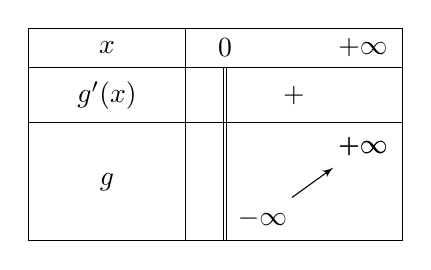
\begin{tikzpicture}[node style/.style={fill opacity=0,text opacity=1}]
        \tkzTabInit[espcl=1.75]{$x$/.5,$g'(x)$/.7,$g$/1.5}{$0$,$+\infty$}
        \tkzTabLine{d,+,}
        \tkzTabVar{D-/$-\infty$,+/$+\infty$/}
    \end{tikzpicture}

\item  Montrons qu'il existe un unique réel $\alpha$ solution de l'équation $g(x) = 0$.\\

En effet, $g$ est continue et strictement croissante sur $]0 ; +\infty[$.\\
Or, $0 \in ]-\infty ; +\infty[$ donc, d'après le théorème de la bijection, il existe un unique réel $\alpha \in ]0 ; +\infty[$ tel que $g(\alpha) = 0$.\\

Vérifions que $\alpha$ appartient à $]0.2 ; 0.3[$.

Soit : $g(0.2) = 1 + 0.2 + \ln 0.2 = -0.40$ et $g(0.3) = 1 + 0.3 + \ln 0.3 = 0.09$.\\
Alors, $g(0.2) \times g(0.3) = -0.36 < 0$.\\

Ainsi, $g$ est continue sur $]0.2 ; 0.3[$ et $g(0.2) \times g(0.3) < 0$.\\

Donc, d'après le corollaire du théorème des valeurs intermédiaires, il existe $\beta \in ]0.2 ; 0.3[$ solution de l'équation $g(x) = 0$.\\
L'unique solution de cette équation est le réel $\alpha$.\\

Par conséquent, $\alpha = \beta$. D'où, $\alpha \in ]0.2 ; 0.3[$.

\item En déduisons le signe de $g$ sur $]0 ; +\infty[$.
D'après les questions précédentes, on peut alors écrire :

\[
g([0 ; \alpha]) = ]-\infty ; 0] \quad \text{et} \quad g([ \alpha ; +\infty[) = [0 ; +\infty[
\]

Ainsi,

\[
g(x) \leq 0 \text{ sur } ]0 ; \alpha[ \quad \text{et} \quad g(x) \geq 0 \text{ sur } [ \alpha ; +\infty[
\]

\item  Établissons la relation $\ln(\alpha) = -1 - \alpha$.

D'après la question 2), $\alpha$ est l'unique solution de l'équation $g(x) = 0$.

Ce qui signifie que $g(\alpha) = 0$.

Par suite,
\[
g(\alpha) = 0 \iff 1 + \alpha + \ln \alpha = 0
\]
\[
\iff \ln \alpha = -1 - \alpha
\]

D'où, la relation :
\[
\ln(\alpha) = -1 - \alpha
\]

\end{enumerate}
\subsection*{\underline{\textbf{Partie B}}:\textbf{ 6,5 pts}}
On considère la fonction $f$ définie par :

\[
f(x) = 
\begin{cases}
\frac{x \ln x}{1 + x} & \text{si } x > 0 \\
0 & \text{si } x = 0
\end{cases}
\]

\begin{enumerate}
    \item Montrons que $f$ est continue en 0 puis sur $]0 ; +\infty[$.

Calculons $\lim\limits_{x \to 0^+} f(x)$.

On a :
\[
\begin{aligned}
\lim\limits_{x \to 0^+} f(x) &= \lim\limits_{x \to 0^+} \frac{x \ln x}{1 + x} \\
&= \lim\limits_{x \to 0^+} \frac{0}{1} \\
&= 0
\end{aligned}
\]

Donc, $\lim\limits_{x \to 0^+} f(x) = f(0)$.

D'où, $f$ est continue en 0.
Par ailleurs, $\forall x_0 \in ]0 ; +\infty[$, $f$ est continue en $x_0$.

Par conséquent, $f$ est continue sur $]0 ; +\infty[$.

\item  Étudions la dérivabilité de $f$ en 0.

Calculons
\[
\lim\limits_{x \to 0^+} \frac{f(x) - f(0)}{x - 0}
\]

On a :
\[
\begin{aligned}
\lim\limits_{x \to 0^+} \frac{f(x) - f(0)}{x} &= \lim\limits_{x \to 0^+} \frac{x \ln x}{(1 + x) x} \\
&= \lim\limits_{x \to 0^+} \frac{x \ln x}{x(1 + x)} \\
&= \lim\limits_{x \to 0^+} \frac{\ln x}{1 + x} \\
&= \lim\limits_{x \to 0^+} \frac{-\infty}{1} \\
&= -\infty
\end{aligned}
\]

Donc,
\[
\lim\limits_{x \to 0^+} \frac{f(x) - f(0)}{x} = -\infty
\]
Ainsi, la fonction $f$ n'est pas dérivable en 0.

Interprétons graphiquement ce résultat.

Comme 
\[
\lim\limits_{x \to 0^+} \frac{f(x) - f(0)}{x - 0} = -\infty,
\]
alors la courbe représentative de $f$ admet une demi-tangente verticale au point d'abscisse 0.

\item Déterminons la limite de $f$ en $+\infty$.

On a :
\[
\begin{aligned}
\lim\limits_{x \to +\infty} f(x) &= \lim\limits_{x \to +\infty} \frac{x \ln x}{1 + x} \\
&= \lim\limits_{x \to +\infty} \frac{x}{x} \times \frac{\ln x}{\frac{1+x}{x}} \\
&= \lim\limits_{x \to +\infty} \frac{\ln x}{\frac{1}{x}+1} \\
&= \lim\limits_{x \to +\infty} \frac{\infty}{0+1} \\
&= +\infty
\end{aligned}
\]

\item Montrons que, quel que soit $x$ élément de $]0 ; +\infty[$. \(f'(x) = \frac{g(x)}{(1 + x)^2}\)

On a : $\forall x \in ]0 ; +\infty[ ; f(x) = \frac{x \ln x}{1 + x}$.

Par suite,

\(
\begin{aligned}
f'(x) &= \frac{(1 + \ln x)(1 + x) - x \ln x}{(1 + x)^2} \\
&= \frac{1 + x + \ln x + x \ln x - x \ln x}{(1 + x)^2} \\
&= \frac{1 + x + \ln x}{(1 + x)^2} \\
&= \frac{g(x)}{(1 + x)^2}
\end{aligned}
\)

Ainsi,
\[
\boxed{f'(x) = \frac{g(x)}{(1 + x)^2}}
\]

En déduisons le signe de $f'(x)$ sur $]0 ; +\infty[$.

Comme $(1 + x)^2 > 0$ alors, le signe de $f'(x)$ dépend uniquement du signe de $g(x)$.

Or, $g(x)$ est négatif sur $]0 ; \alpha[$ et positif sur $[\alpha ; +\infty[$.

Par conséquent,
\begin{itemize}
    \item \(f'(x) \leq 0 \text{ sur } ]0 ; \alpha[\)
    \item  \(f'(x) \geq 0 \text{ sur } [\alpha ; +\infty[\)
\end{itemize}

\item  Montrons que $f(\alpha) = -\alpha$.

Soit : 
\(f(\alpha) = \frac{\alpha \ln \alpha}{1 + \alpha}\)

Or, dans la première partie, à la question 4), on avait : $\ln \alpha = -1 - \alpha$.

Donc, en remplaçant $\ln \alpha$ par son expression, on obtient :

\(
\begin{aligned}
f(\alpha) &= \frac{\alpha \ln \alpha}{1 + \alpha}\\
&= \frac{\alpha (-1 - \alpha)}{1 + \alpha} \\
&= \frac{-\alpha(1 + \alpha)}{1 + \alpha} \\
&= -\alpha
\end{aligned}\)

Ainsi,
\(\boxed{f(\alpha) = -\alpha}\)

\item Dressons le tableau de variations de la fonction f.

    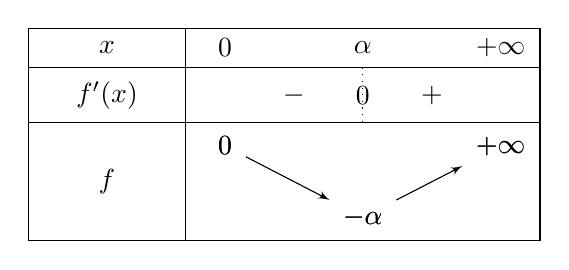
\begin{tikzpicture}[node style/.style={fill opacity=0,text opacity=1}]
        \tkzTabInit[espcl=1.75]{$x$/.5,$f'(x)$/.7,$f$/1.5}{$0$,$\alpha$,$+\infty$}
        \tkzTabLine{,-,z,+}
        \tkzTabVar{+/$0$,-/$-\alpha$,+/$+\infty$/}
    \end{tikzpicture}
    
\item Représentons la courbe de $f$ dans le plan muni du repère orthonormal $(O ; \vec{i}, \vec{j})$. Unité graphique : 5 cm. Prendre $\alpha \approx 0.3$.

% Insérer l'image
\begin{figure}[h!]
    \centering
    \includegraphics[width=0.8\textwidth]{devoir4.png} % Remplacez par le chemin de votre image
    \label{fig:courbe_f}
\end{figure}

\end{enumerate}

\end{document}